% Template of basic phisics experiment 基于 article template, 在此基础上做修改
% 设定文章编码类型, 正文字号为五号则 zihao=5, 正文字号为小四则 zihao=-4
\documentclass[zihao=5, UTF8]{article}		


% 自定义宏定义
\def\N{\mathbb{N}}
\def\F{\mathbb{F}}
\def\Z{\mathbb{Z}}
\def\Q{\mathbb{Q}}
\def\R{\mathbb{R}}
\def\C{\mathbb{C}}
\def\T{\mathbb{T}}
\def\S{\mathbb{S}}
\def\A{\mathbb{A}}
\def\I{\mathscr{I}}
\def\d{\mathrm{d}}
\def\p{\partial}


% 物理实验报告所需的其它宏包
\usepackage{ulem}   % \uline 下划线支持

% 导入基本宏包
\usepackage[UTF8]{ctex}     % 设置文档为中文语言
\usepackage[colorlinks, linkcolor=blue, anchorcolor=blue, citecolor=blue, urlcolor=blue]{hyperref}  % 宏包：自动生成超链接 (此宏包与标题中的数学环境冲突)
% \usepackage{docmute}    % 宏包：子文件导入时自动去除导言区, 用于主/子文件的写作方式, \include{./51单片机笔记}即可. 注：启用此宏包会导致.tex文件capacity受限. 
\usepackage{amsmath}    % 宏包：数学公式
\usepackage{physics}
\usepackage{bm}
\usepackage{mathrsfs}   % 宏包：提供更多数学符号
\usepackage{amssymb}    % 宏包：提供更多数学符号
\usepackage{pifont}     % 宏包：提供了特殊符号和字体
\usepackage{extarrows}  % 宏包：更多箭头符号
\usepackage{multirow}
\usepackage{siunitx}

\renewcommand{\dd}{\mathrm{d}}

% 列表环境设置
\usepackage{enumitem}   % 宏包：列表环境设置
    \setlist[enumerate]{itemsep=0pt, parsep=0pt, topsep=0pt, partopsep=0pt, leftmargin=3.5em} 
    \setlist[itemize]{itemsep=0pt, parsep=0pt, topsep=0pt, partopsep=0pt, leftmargin=3.5em}
    \newlist{circledenum}{enumerate}{1} % 创建一个新的枚举环境  
    \setlist[circledenum,1]{  
        label=\protect\circled{\arabic*}, % 使用 \arabic* 来获取当前枚举计数器的值, 并用 \circled 包装它  
        ref=\arabic*, % 如果需要引用列表项, 这将决定引用格式（这里仍然使用数字）
        itemsep=0pt, parsep=0pt, topsep=0pt, partopsep=0pt, leftmargin=3.5em
    }  
% 文章页面 margin 设置
\usepackage[a4paper]{geometry}  % 宏包：文章页面 margin 设置
    \geometry{top=0.75in}
    \geometry{bottom=0.75in}
    \geometry{left=0.75in}
    \geometry{right=0.75in}   % 设置上下左右页边距
    \geometry{marginparwidth=1.75cm}    % 设置边注距离（注释、标记等）

% 自定义数学环境
\usepackage{amsthm} % 宏包：数学环境配置
% theorem-line 环境自定义
    \newtheoremstyle{MyLineTheoremStyle}% <name>
        {11pt}% <space above>
        {11pt}% <space below>
        {}% <body font> 使用默认正文字体
        {}% <indent amount>
        {\bfseries}% <theorem head font> 设置标题项为加粗
        {：}% <punctuation after theorem head>
        {.5em}% <space after theorem head>
        {\textbf{#1}\thmnumber{#2}\ \ (\,\textbf{#3}\,)}% 设置标题内容顺序
    \theoremstyle{MyLineTheoremStyle} % 应用自定义的定理样式
    \newtheorem{LineTheorem}{Theorem.\,}
% theorem-block 环境自定义
    \newtheoremstyle{MyBlockTheoremStyle}% <name>
        {11pt}% <space above>
        {11pt}% <space below>
        {}% <body font> 使用默认正文字体
        {}% <indent amount>
        {\bfseries}% <theorem head font> 设置标题项为加粗
        {：\\ \indent}% <punctuation after theorem head>
        {.5em}% <space after theorem head>
        {\textbf{#1}\thmnumber{#2}\ \ (\,\textbf{#3}\,)}% 设置标题内容顺序
    \theoremstyle{MyBlockTheoremStyle} % 应用自定义的定理样式
    \newtheorem{BlockTheorem}[LineTheorem]{Theorem.\,} % 使用 LineTheorem 的计数器
% definition 环境自定义
    \newtheoremstyle{MySubsubsectionStyle}% <name>
        {11pt}% <space above>
        {11pt}% <space below>
        {}% <body font> 使用默认正文字体
        {}% <indent amount>
        {\bfseries}% <theorem head font> 设置标题项为加粗
        {：\\ \indent}% <punctuation after theorem head>
        {0pt}% <space after theorem head>
        {\textbf{#3}}% 设置标题内容顺序
    \theoremstyle{MySubsubsectionStyle} % 应用自定义的定理样式
    \newtheorem{definition}{}


% 有色文本框及其设置
\usepackage[dvipsnames,svgnames]{xcolor}    %设置插入的文本框颜色
\usepackage[strict]{changepage}     % 提供一个 adjustwidth 环境
\usepackage{framed}     % 实现方框效果
    \definecolor{graybox_color}{rgb}{0.95,0.95,0.96} % 文本框颜色. 修改此行中的 rgb 数值即可改变方框纹颜色, 具体颜色的rgb数值可以在网站https://colordrop.io/ 中获得. （截止目前的尝试还没有成功过, 感觉单位不一样）（找到喜欢的颜色, 点击下方的小眼睛, 找到rgb值, 复制修改即可）
    \newenvironment{graybox}{%
    \def\FrameCommand{%
    \hspace{1pt}%
    {\color{gray}\small \vrule width 2pt}%
    {\color{graybox_color}\vrule width 4pt}%
    \colorbox{graybox_color}%
    }%
    \MakeFramed{\advance\hsize-\width\FrameRestore}%
    \noindent\hspace{-4.55pt}% disable indenting first paragraph
    \begin{adjustwidth}{}{7pt}%
    \vspace{2pt}\vspace{2pt}%
    }
    {%
    \vspace{2pt}\end{adjustwidth}\endMakeFramed%
    }

% 各级标题自定义设置
\usepackage{titlesec}   
    % section标题自定义设置 
    \titleformat{\section}[hang]{\normalfont\huge\bfseries\centering}{第\,\thesection\,部分}{20pt}{}
    % subsection标题自定义设置 
    \titleformat{\subsection}[hang]{\normalfont\Large\bfseries}{\,\thesubsection\,}{8pt}{}
    % subsubsection标题自定义设置
    \titleformat{\subsubsection}[hang]{\normalfont\large\bfseries}{\,\thesubsubsection\,}{6pt}{}

% 外源代码插入设置
\usepackage{matlab-prettifier}
    \lstset{
        style=Matlab-editor,  % 继承matlab代码颜色等
    }
\usepackage[most]{tcolorbox} % 引入tcolorbox包 
\usepackage{listings} % 引入listings包
    \tcbuselibrary{listings, skins, breakable}
    \lstdefinestyle{matlabstyle}{
        language=Matlab,
        basicstyle=\small,
        breakatwhitespace=false,
        breaklines=true,
        captionpos=b,
        keepspaces=true,
        numbers=left,
        numbersep=15pt,
        showspaces=false,
        showstringspaces=false,
        showtabs=false,
        tabsize=2
    }
    \newtcblisting{matlablisting}{
        arc=0pt,
        top=0pt,
        bottom=0pt,
        left=1mm,
        listing only,
        listing style=matlabstyle,
        breakable,
        colback=white   % 选一个合适的颜色
    }

% table 支持
\usepackage{booktabs}   % 宏包：三线表
\usepackage{tabularray} % 宏包：表格排版
\usepackage{longtable}  % 宏包：长表格

% figure 设置
\usepackage{graphicx}  % 支持 jpg, png, eps, pdf 图片 
\usepackage{svg}       % 支持 svg 图片
    \svgsetup{
        % 指向 inkscape.exe 的路径
        inkscapeexe = C:/aa_MySame/inkscape/bin/inkscape.exe, 
        % 一定程度上修复导入后图片文字溢出几何图形的问题
        inkscapelatex = false                 
    }


% 图表进阶设置
\usepackage{float}     % 图表位置浮动设置 
\usepackage{caption}    % 图注、表注
    \captionsetup[figure]{name=图}  
    \captionsetup[table]{name=表}
    \captionsetup{labelfont=bf, font=small}

%% 文章默认字体设置
%    \usepackage{fontspec}   % 宏包：字体设置
%        \setmainfont{SimSun}[
%            BoldFont = SimHei, % 设置粗体字为黑体
%            ItalicFont = KaiTi, % 设置斜体字为楷体
%            BoldItalicFont = KaiTi % 设置粗斜体字为楷体
%        ] 
%        %\setCJKmainfont[AutoFakeBold=3]{SimSun} % 设置加粗字体为 SimSun 族, AutoFakeBold 可以调整字体粗细
%        \setmainfont{Times New Roman} % 设置英文字体为Times New Roman


% 其它设置
    % equation 公式编号设置
        \makeatletter  
        \renewcommand{\theequation}{\thesection.\arabic{equation}}  
        \makeatother
    % 脚注设置
        \renewcommand\thefootnote{\ding{\numexpr171+\value{footnote}}}
    % 参考文献引用设置
        \bibliographystyle{unsrt}   % 设置参考文献引用格式为unsrt
        \newcommand{\upcite}[1]{\textsuperscript{\cite{#1}}}     % 自定义上角标式引用
    % 文章序言设置
        \newcommand{\cnabstractname}{序言}
        \newenvironment{cnabstract}{%
            \par\Large
            \noindent\mbox{}\hfill{\bfseries \cnabstractname}\hfill\mbox{}\par
            \vskip 2.5ex
            }{\par\vskip 2.5ex}


% 页眉页脚设置
\usepackage{fancyhdr}   %宏包：页眉页脚设置
    \pagestyle{fancy}
    \fancyhf{}
    \cfoot{\thepage}
    \renewcommand\headrulewidth{1pt}
    \renewcommand\footrulewidth{0pt}
    \rhead{\bfseries 分组序号: 3-04-1}    
    \chead{《基础物理实验》实验报告,\ 潘天麟\ 2023K8009908023}
    \lhead{2024.11.20}

\usepackage{pdfpages}

% 开始编辑文章

\begin{document}
\noindent\begin{flushright}
    \zihao{2}{分组序号: 3-04-1}
\end{flushright}

\newcommand*{\boldsong}{\CJKfamily{boldsong}}


\begin{center}\large
    \noindent{\Huge\bfseries\boldsong《基础物理实验》实验报告 }
    \\\vspace{0.4cm}
    \noindent\textit{
        \textbf{\boldsong 实验名称：}\uline{\hspace{2.3cm} 热导温度测量\hspace{2.3cm}}\hspace{0.4cm} 
        指导教师：\uline{\hspace{1.5cm}赵同宪\hspace{1.5cm}}}
    \\\vspace{0.1cm}
    \noindent\textit{
        姓名：\uline{\,\,潘天麟\,\,}\hspace{0.2cm}
        学号：\uline{\,\,{\upshape 2023K8009908023}\,\,}\hspace{0.2cm}
        专业：\uline{\,\,人工智能\,\,}\hspace{0.2cm}
        班级：\uline{\,\,\upshape{2313}\,\,}\,组号：\uline{\,\,\upshape{3-04-1}\,\,}}
    \\\vspace{0.1cm}
    \noindent\textit{
        实验日期：\uline{\,\,{\upshape 2024.11.20}\,\,}\hspace{0.2cm}
        实验地点：\uline{\,\,\,教学楼{\upshape 427}\,\,\,}\hspace{0.2cm}
        是否调课/补课：\uline{\,\,否\,\,}\hspace{0.2cm}
        成绩：\uline{\hspace{2cm}}}
\end{center}
% \vspace{-0.2cm}
\noindent\rule{\textwidth}{0.1em}   % 分割线

% 控制目录不换页
\vspace{1cm}
\setcounter{tocdepth}{3}  % 目录深度为 2（不显示 subsubsection）
\noindent\begin{minipage}{\textwidth}\centering
\tableofcontents\thispagestyle{fancy}   % 显示页码、页眉等   
\end{minipage}  
\newpage
\section{动态法测定良导体的热导率}
\subsection{实验目的}
\begin{enumerate}
    \item 通过实验学会一种测量热导率的方法
    \item 了解动态法的特点和优越性. 
    \item 认识热波, 加强对波动理论的理解. 
\end{enumerate}
\subsection{实验仪器}
\begin{enumerate}
    \item 热导率动态测量仪
    \item 铜棒, 铝棒
    \item 计算机
\end{enumerate}
\subsection{实验原理}
由热传导定律, 单位时间内流过某垂直于传播方向上面元$A$的热量$q$满足
\begin{equation}
    \frac{\dd q}{\dd t} = -kA \frac{\dd T}{\dd x},
\end{equation}
其中$k$为待测材料的热导率, $A$为截面积, $\frac{\dd T}{\dd x}$是温度对坐标$x$的梯度. 式子两边同时取微分可以得到
\begin{equation}
    \dd\left(\frac{\dd q}{\dd t}\right) = -kA \frac{\dd^2T}{\dd x^2} \dd x.
\end{equation}
根据能量守恒定律, 任一时刻棒元的热平衡方程为：
\begin{equation}
    C\rho A \dd x \frac{\dd T}{\dd t} = \dd\left(\frac{\dd q}{\dd t}\right) = -kA \frac{\dd^2T}{\dd x^2} \dd x,
\end{equation}
其中$C$为材料的比热容, $\rho$为材料的密度. 故热流方程为
\begin{equation}
    \frac{\dd T}{\dd t} = D \frac{\dd^2 T}{\dd x^2}.
\end{equation}
则可知棒中温度呈简谐变化, 一端温度恒定, 另一端用冷水冷却, 则可得到
\begin{equation}
    T = T_0 - \alpha x + T_m e^{-\sqrt{\omega / 2D} x} \sin(\omega t - \sqrt{\omega / 2D} x),
\end{equation}
从中可以看出热波波速$v$满足
\begin{equation}
    v = \sqrt{2D\omega}.
\end{equation}
从而我们可以计算材料的热导率
\begin{equation}
    k = \frac{v^2 C \rho}{4\pi f} = \frac{v^2 C \rho}{4\pi T}
\end{equation}
\subsection{实验内容}
\begin{enumerate}
    \item 打开水龙头至大约三分之一处, 使得冷水出水恒定
    \item 打开电源开关, 使得热导率动态测量仪进入工作状态
    \item 打开热导率动态测量仪连接的电脑, 打开电脑中的对应操作软件, 设置周期为180秒, 选择测试样品, 点击测量按钮开始测量, 等到图样达到平衡状态之后点击暂停, 并且导出数据
    \item 在两个样品均测量完毕后, 先关闭热导率动态测量仪, 再关闭水龙头, 最后将数据文件发送至自己的电脑上
\end{enumerate}
\subsection{实验数据及处理}
\subsubsection{动态法测铜的热导率}
\begin{table}[H]
\centering
\begin{tabular}{|c|c|c|c|c|c|c|} 
\hline
测量点$n$       & 1       & 2       & 3       & 4       & 5       & 6        \\ 
\hline
对应峰值时间$t$(s) & 2409.04 & 2443.52 & 2451.52 & 2460.52 & 2470.04 & 2476.52  \\ 
\hline
波速$v$(m/s)   & 4.46$\times 10^{-3}$    & 2.50$\times 10^{-3}$    & 2.22$\times 10^{-3}$    & 2.10$\times 10^{-3}$    & 3.08$\times 10^{-3}$    & ~        \\ 
\hline
\multicolumn{3}{|c|}{波速平均值: 2.87$\times 10^{-3}$ m/s}  & \multicolumn{4}{c|}{热导率: 405 W/mK}                \\
\hline
\end{tabular}
\caption{动态法测铜的热导率}
\label{tab:cu}
\end{table}
 
在表\ref{tab:cu}中, 相邻热电偶的间距为$l_0 = 2$cm, 通过$v_n = \dfrac{l_0}{t_{n+1}- t_{n}}$, 计算波速如下
\begin{gather}
    v_1 = \frac{0.02}{2443.52 - 2409.04} = 4.46\times 10^{-3}\text{m/s},\\
    v_2 = \frac{0.02}{2451.52 - 2443.52} = 2.50\times 10^{-3}\text{m/s},\\
    v_3 = \frac{0.02}{2460.52 - 2451.52} = 2.22\times 10^{-3}\text{m/s},\\
    v_4 = \frac{0.02}{2470.04 - 2460.52} = 2.10\times 10^{-3}\text{m/s},\\
    v_5 = \frac{0.02}{2476.52 - 2470.04} = 3.08\times 10^{-3}\text{m/s}.
\end{gather}
从而可计算平均波速为
\begin{equation}
    v = \frac{4.46\times 10^{-3} + 2.50\times 10^{-3} + 2.22\times 10^{-3} + 2.10\times 10^{-3} + 3.08\times 10^{-3}}{5} = 2.87\times 10^{-3}\text{m/s}.
\end{equation}
代入铜的比热$C = 0.385$J/gK, 密度$8.92$g/cm$^3$, 可计算铜的热导率为
\begin{equation}
    k = \frac{v^2 C \rho}{4\pi f} = 405\text{W/mK}.
\end{equation}

原始数据绘图如下
\begin{figure}[H]
    \centering
    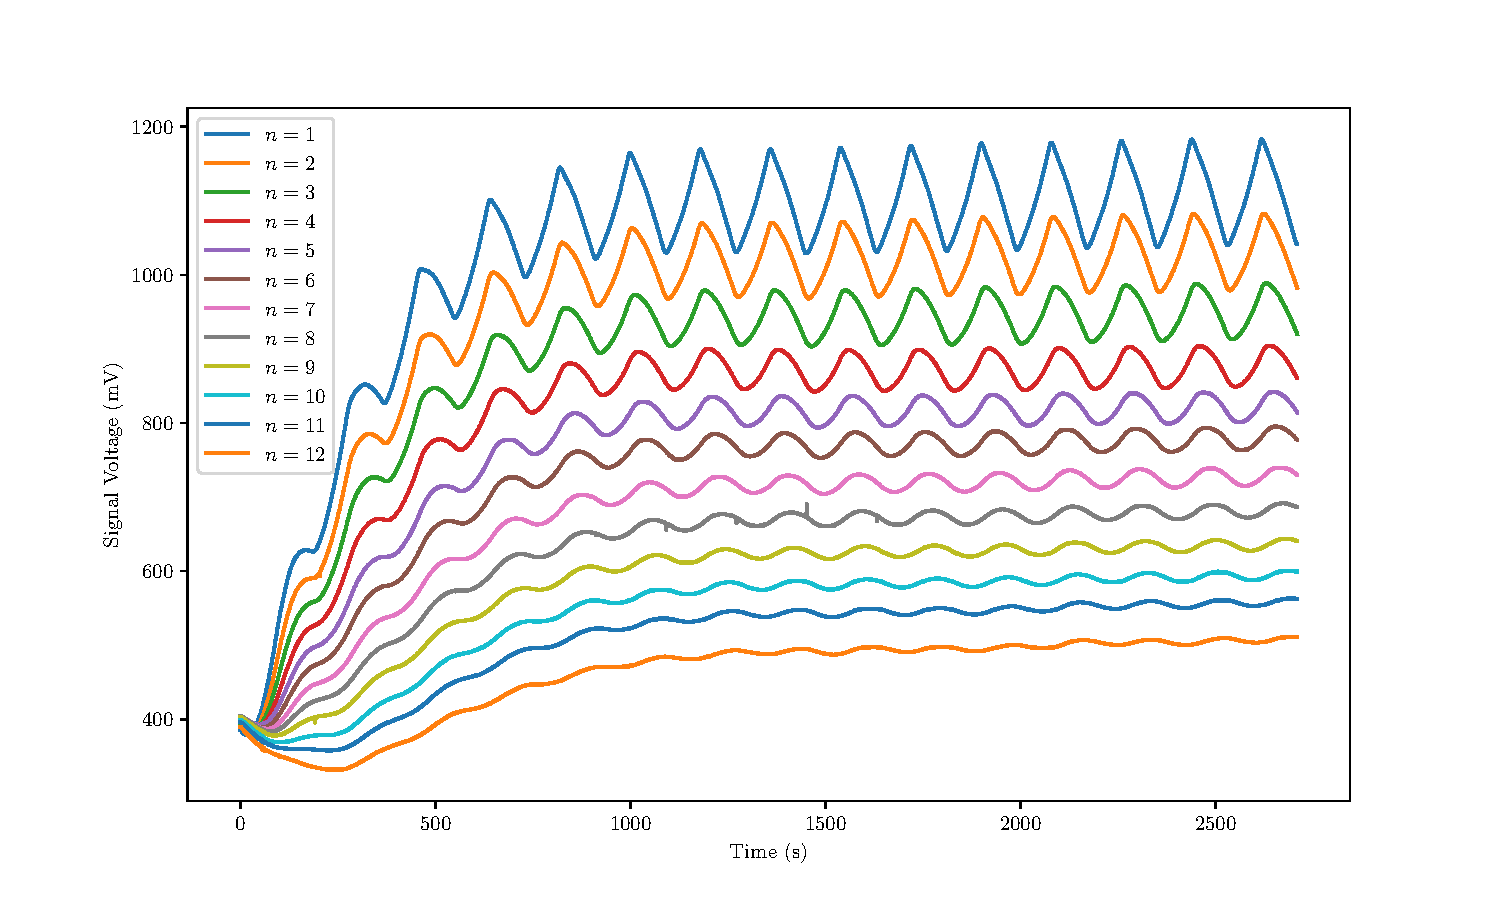
\includegraphics[width=0.9\textwidth]{Cu-data.pdf}
    \caption{铜的热导率测量}
    \label{fig:cu}
\end{figure}

\subsubsection{动态法测铝的热导率}
\begin{table}[H]
\centering
\begin{tabular}{|c|c|c|c|c|c|c|} 
\hline
测量点$n$       & 1       & 2       & 3       & 4       & 5       & 6        \\ 
\hline
对应峰值时间$t$(s) & 2274.04 & 2286.04 & 2295.52 & 2305.04 & 2314.04 & 2325.52  \\ 
\hline
波速$v$(m/s)   & 1.67$\times 10^{-3}$    & 2.11$\times 10^{-3}$    & 2.10$\times 10^{-3}$    & 2.22$\times 10^{-3}$    & 1.74$\times 10^{-3}$    & ~        \\ 
\hline
\multicolumn{3}{|c|}{波速平均值: 1.97$\times 10^{-3}$ m/s}  & \multicolumn{4}{c|}{热导率: 135 W/mK}                \\
\hline
\end{tabular}
\caption{动态法测铝的热导率}
\label{tab:al}
\end{table}

同样地, 在表\ref{tab:al}中, 相邻热电偶的间距为$l_0 = 2$cm, 通过$v_n = \dfrac{l_0}{t_{n+1}- t_{n}}$, 计算波速如下
\begin{gather}
    v_1 = \frac{0.02}{2286.04 - 2274.04} = 1.67\times 10^{-3}\text{m/s},\\
    v_2 = \frac{0.02}{2295.52 - 2286.04} = 2.11\times 10^{-3}\text{m/s},\\
    v_3 = \frac{0.02}{2305.04 - 2295.52} = 2.10\times 10^{-3}\text{m/s},\\
    v_4 = \frac{0.02}{2314.04 - 2305.04} = 2.22\times 10^{-3}\text{m/s},\\
    v_5 = \frac{0.02}{2325.52 - 2314.04} = 1.74\times 10^{-3}\text{m/s}.
\end{gather} 

从而可计算平均波速为
\begin{equation}
    v = \frac{1.67\times 10^{-3} + 2.11\times 10^{-3} + 2.10\times 10^{-3} + 2.22\times 10^{-3} + 1.74\times 10^{-3}}{5} = 1.97\times 10^{-3}\text{m/s}.
\end{equation}

代入铝的比热$C = 0.90$J/gK, 密度$2.70$g/cm$^3$, 可计算铝的热导率为
\begin{equation}
    k = \frac{v^2 C \rho}{4\pi f} = 135\text{W/mK}.
\end{equation}

原始数据绘图如下
\begin{figure}[H]
    \centering
    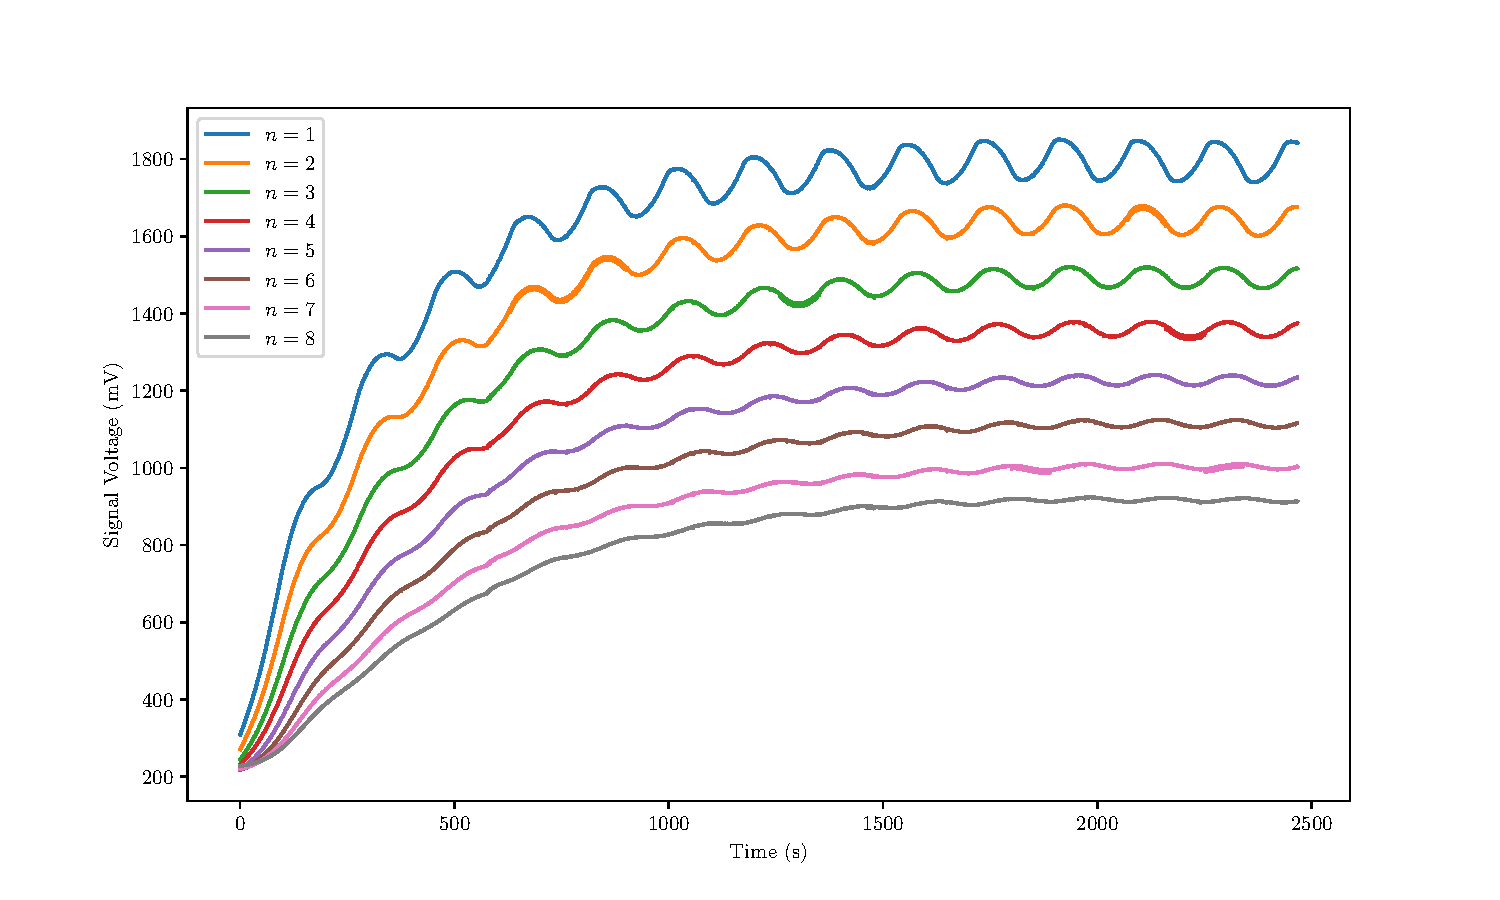
\includegraphics[width=0.9\textwidth]{Al-data.pdf}
    \caption{铝的热导率测量}
    \label{fig:al}
\end{figure}
\subsection{思考题}
\textbf{如何获得某一时刻 $t$ 时材料棒上的热波, 即 $T \sim x$ 曲线？}

在被测材料上每隔一段距离放置热电偶传感器, 并且记录下在的$t$时刻它们的信号读数, 根据信号值与温度的对应关系求出实际的温度读书, 
将不同测量点上测得的温度连接得到所求曲线. 此外也可以将之前实验中求得的热导率代入公式
\begin{equation}
T = T_0 - \alpha x + T_m e^{-\sqrt{\frac{\omega}{2D}} x} \sin(\omega t - \sqrt{\frac{\omega}{2D}} x)
\label{eq:curve}
\end{equation}
由此可作图得到所求曲线. 

\textbf{为什么较后面测量点的 $T \sim t$ 曲线振幅越来越小？}

根据公式\ref{eq:curve}, $x$越大, $e^{-\sqrt{\frac{\omega}{2D}} x}$越小, 即简谐运动的振幅越小

\textbf{为什么实验中铝棒的测温点只有 8 个, 而铜棒的测温点达到 12 个？}

由于热扩散系数$D$正比于热导率$k$, 且铝的热导率比铜的要小, 所以铝的热扩散系数$D$比铜更小, 
从而铝的$e^{-\sqrt{\frac{\omega}{2D}} x}$振幅项的衰减速度更快. 
所以只需取8个测量点即可观察到显著的振幅差异. 
这时候如果取更多的测量点, 由于振幅的衰减, 后面的测量点的振幅会非常小, 所以没有太大的必要

\textbf{实验中误差的来源有哪些？}

实验中可能出现的误差来源可能有
\begin{enumerate}
    \item 热容和密度参考值不能准确反映被测材料的实际情况 
    \item 判断峰值时间的准确性
    \item 热电偶的间隔位置的误差
    \item 热电偶本身的系统误差
\end{enumerate}
\subsection{心得体会}
这部分的实验基本由热导率动态测量仪自动完成, 在实际实验中我们只需要设置好参数, 打开水龙头, 点击测量按钮, 等待数据采集完毕即可.
但是收集数据时间比较漫长, 为了最大化时间利用率, 我们可以在等待数据采集的时候进行其他实验的准备工作, 以提高实验效率.

处理实验数据的时候我们需要找出每一个峰值对应的时间, 但是由于热电偶传感器的测量精度有限, 在靠近峰值的部分常常会出现
读数在两个间隔为最小测量精度的数字之间摆动, 这时候比较难以准确地判断峰值时间. 对此我的解决方案是对相邻的两个数据点进行差分,
之后再对差分数据进行平滑处理:

\begin{equation}
    \Delta V_t = V_{t + \Delta t} - V_t, \quad \Delta \tilde{V}_t = 
    \dfrac{\sum_{\tau = t -T_0}^{t + T_0} w(\tau - t)\Delta V_t}{\sum_{\tau = t -T_0}^{t + T_0} w(\tau - t)}
\end{equation}
其中取高斯形式的$w(\tau - t)$为权重函数(这里取$\sigma = 1$)
\begin{equation}
    w(\tau - t) = \frac{1}{\sqrt{2\pi}\sigma}e^{-\frac{(\tau - t)^2}{2\sigma^2}}
\end{equation}

最后我们取平滑差分函数$\Delta \tilde{V}_t$的零点作为真正的峰值时间. 通过这种方法, 我们可以减小由于测量精度带来的误差.

就最后的结果而言, 使用这种处理办法得到的铜的热导率(405 W/mK)和参考值(401 W/mK)相差不大, 但是率的热导率
(135 W/mK)和参考值(237 W/mK)相差较大. 我参考了其他同学的实验报告, 发现他们的结果也是有较大的偏小的误差,
这可能是由于实验中某些环境因素或者是使用的被测铝材自身的问题导致的. 但是总的来说, 这次实验还是比较成功的.
\section{温度的测量和温度计的设计}
\subsection{实验目的}
\begin{enumerate}
    \item 用电位差计测热电偶的温差电动势. 
    \item 用平衡电桥测热敏电阻和铜电阻的温度特性曲线. 
    \item 设计非平衡电桥实现对热敏电阻的实时测量. 
\end{enumerate}

\subsection{实验仪器}
\begin{itemize}
    \item DHT-2型热学实验仪
    \item DHQJ-5型教学用多功能电桥
    \item UJ36a型携带式直流电位差计
    \item 保温瓶
    \item 导线
    \item 冰水混合物
\end{itemize}

\subsection{实验原理}
\subsubsection{用电位差计测热电偶的温差电动势}
热电偶是由两种不同材料的金属丝的端点紧密接触组成的. 当两个接点温度不同时, 就会有直流电动势产生, 即温差电动势. 当组成热电偶的材料确定时, 两接点的温差与温差电动势之间存在以下近似关系式：
\begin{equation}
    E_x \approx \alpha (t - t_0)
\end{equation}
其中 $\alpha$ 被称为热温差系数, 在已知温差和温差电动势的情况下就可以计算出热温差系数. 

\subsubsection{用平衡电桥测电阻的温度特性曲线}
在温度不是很高时, 金属的电阻值可以视为随温度近似线性变化, 即：
\begin{equation}
    R_x = R_{x0} (1 + \alpha t)
\end{equation}
其中 $R_{x0}$ 是在 $t = 0^\circ C$ 时的电阻值. 通过在一系列温度下使用平衡电桥测量金属的电阻值, 可以绘制出金属的温度特性曲线并求得温度系数 $\alpha$. 

对于半导体, 其电阻值可以用以下公式描述：
\begin{equation}
    R_T = A e^{B/T}
\end{equation}
这里 $A$ 是与材料性质和电阻器几何形状相关的常数, $B$ 是与材料半导体性质相关的常数, $T$ 是绝对温度. 对两边同时取自然对数后可得 $\ln R_T$ 与 $1/T$ 呈线性关系. 绘制这两者之间的线性关系图, 可以通过求解直线方程来计算出 $A$ 和 $B$ 的值. 

\subsubsection{设计非平衡电桥实现对热敏电阻的实时测量}
对于非平衡电桥, 假设电压表的内阻无穷大, 并忽略流过电压表的电流, 则 $U_0$ 满足以下关系：
\begin{equation}
    U_0 = \left(\frac{R_x}{R_1 + R_x} - \frac{R_1}{R_1 + R_3}\right) E
\end{equation}
将上式进行泰勒展开, 保留至二阶项, 得到：
\begin{equation}
    U_0 = U_{01} + U'_0 (T - T_1) + U''_0 (T - T_1)^2
\end{equation}
取 $T_1 = 40^\circ C$, 令 $U''_0 = 0$, 则有：
\begin{equation}
    R_x = \frac{B + 2T}{B - 2T} R_2
\end{equation}
因此, $U_0$ 可以表示为 $T$ 的线性表达式：
\begin{equation}
    U_0 = \lambda + m(t - t_1)
\end{equation}
并且有：
\begin{gather}
    E = \frac{4 B T_1^2}{4 T_1^2 - B^2} m, \quad R_2 = \frac{B - 2T}{B + 2T} R_x T_1 \\
    \frac{R_1}{R_3} = \frac{2 B E}{(B + 2 T_1) E - 2 B \lambda} - 1
\end{gather}
通过上述公式可以计算出 $E$, $R_1$, $R_2$, $R_3$ 的值. 将电路中相应的值设置好后, 可以改变设定温度并观察测试电压, 进而根据公式计算出的测试电压来计算测试温度与实际温度之间的误差. 

\subsection{实验内容}

\subsubsection{用电位差计测热电偶的温差电动势}
在室温下测量热电偶的温差电动势, 然后打开温控仪电源, 对热端加热, 在$30\si{\celsius}$到$50\si{\celsius}$的区间内每隔$5\si{\celsius}$进行一次测量并且记录数据. 

\subsubsection{用平衡电桥测电阻的温度特性曲线}
在室温下通过平衡电桥测量铜电阻与半导体电阻的电阻值, 然后在测量温差电动势的同时进行铜电阻与半导体电阻阻值的测量, 测量范围同上. 

\subsubsection{设计非平衡电桥实现对热敏电阻的实时测量}
在上一个实验中利用热敏电阻测量出来的数据计算出$A$与$B$, 根据已知的表头参数以及上述公式计算出$E$, $R_1$, $R_2$, $R_3$的值, 将温控仪温度调至40\si{\celsius}后, 微调$R_1$使得电压表电压趋近于-400mV, 随后在40\si{\celsius}到50\si{\celsius}的区间内以每2\si{\celsius}测量一次为间隔测量5组测试电压以及计算出测试温度与设定温度进行比较. 

\subsection{实验数据及处理}
\subsubsection{用电位差计测热电偶的温差电动势}
保持冷端温度在$t_0 = 0\si{\celsius}$, 测量得到的热电偶温差电动势与温度的关系如表\ref{tab:thermocouple}所示
\begin{table}[H]
\centering
\begin{tabular}{|c|c|c|c|c|c|} 
\hline
温度$t(\si{\celsius})$  & 30.2  & 35.1  & 40.2  & 45.0  & 50.0   \\ 
\hline
电动势$E_x(\si{\milli\volt})$ & 0.768 & 0.966 & 1.034 & 1.060 & 1.082  \\
\hline
\end{tabular}
\caption{用电位差计测热电偶的温差电动势}
\label{tab:thermocouple}
\end{table}

对数据进行线性拟合, 得到的拟合直线如图\ref{fig:thermocouple}所示
\begin{figure}[H]
    \centering
    
\includegraphics[width=0.9\textwidth]{plot3.pdf}
    \caption{热电偶温差电动势与温度的关系}
    \label{fig:thermocouple}
\end{figure}

可以发现一方面$R^2$值不够高, 只有0.8; 另一方面所求的温差电系数$\alpha = 0.01$和其他
同学的结果相差较大. 我注意到在实验过程中, 有一次测量后我检查一下冰水混合物的情况,
发现大部分冰已经融化, 所以这个时候测量的温度可能不够准确, 这可能是导致误差的原因之一.
另一方面我发现在实验中稍微移动热电偶在冰水混合物中的位置, 电动势的读数会有较大的波动, 待稳定后
又和最初的示数不同, 这也可能会导致我测量的误差

\subsubsection{用平衡电桥测电阻的温度特性曲线}

测量得到的铜电阻值和温度的关系如表\ref{tab:copper-resistor}所示
\begin{table}[H]
\centering
\begin{tabular}{|c|c|c|c|c|c|} 
\hline
温度$t(\si{\celsius})$ & 30.0 & 35.0 & 40.0 & 45.0 & 50.0  \\ 
\hline
电阻$R_x(\si{\ohm})$ & 58.2 & 59.4 & 60.5 & 61.5 & 62.7  \\
\hline
\end{tabular}
\caption{铜电阻阻值随温度变化的关系}
\label{tab:copper-resistor}
\end{table}

我们对数据进行线性拟合, 得到的拟合直线如图\ref{fig:copper-resistor}所示
\begin{figure}[H]
    \centering
    
\includegraphics[width=0.9\textwidth]{plot4.pdf}
    \caption{铜电阻阻值随温度变化的关系}
    \label{fig:copper-resistor}
\end{figure}

可以发现拟合直线的$R^2$值为1.00, 说明拟合效果很好, 由于
\begin{equation}
    R_x = 0.22t + 51.58 = 51.58(1 + 0.00425t) 
\end{equation}
由此得到铜的温度系数$\alpha = 4.25 \times 10^{-3}\si{\per\celsius}$, 
这个值和参考值($4.29 \times 10^{-3}\si{\per\celsius}$)非常接近, 说明实验结果是比较准确的.
\newline
\newline
\par
测量得到的热敏电阻值和温度的关系如表\ref{tab:thermistor}所示
\begin{table}[H]
\centering
\begin{tabular}{|c|c|c|c|c|c|} 
\hline
温度$t(\si{\celsius})$ & 30.0 & 35.0 & 40.0 & 45.0 & 50.0  \\ 
\hline
电阻$R_x(\si{\ohm})$ & 2209.2 & 1789.4 & 1461.5 & 1199.5 & 989.1  \\
\hline
\end{tabular}
\caption{热敏电阻阻值随温度变化的关系}
\label{tab:thermistor}
\end{table}

对电阻阻值取对数后, 和倒数温度进行线性拟合, 如图\ref{fig:thermistor}所示
\begin{figure}[H]
    \centering
    
\includegraphics[width=0.9\textwidth]{plot5.pdf}
    \caption{热敏电阻阻值随温度变化的关系}
    \label{fig:thermistor}
\end{figure}

可以发现决定系数$R^2$值为1.00, 说明拟合效果很好, 
由此得到热敏电阻的特性常数$A = 5.158 \times 10^{-3}$, $B = 3.929 \times 10^3$

并取$\lambda = -0.4\mathrm{V}$, $m = -0.01\si{\volt \per \celsius}$, 计算相关参数
\begin{gather}
    E = \dfrac{4 B T_1^2}{4 T_1^2 - B^2} m = 1.023\text{V},\\
    R_2 = \dfrac{B - 2T}{B + 2T} R_x T_1 = 1059.8\Omega,\\
    \dfrac{R_1}{R_3} = \dfrac{2 B E}{(B + 2 T_1) E - 2 B \lambda} - 1 = 3.03 \times 10^{-2}.
\end{gather}

\subsubsection{设计非平衡电桥实现对热敏电阻的实时测量}
根据上述参数调整非平衡电桥, 最终电阻取值为$R_1 = 30.3 \Omega$, $R_2 = 1012.8 \Omega$, $R_3 = 1000 \Omega$.
由此测量$40\si{\celsius} \sim 50\si{\celsius}$的温度, 测量数据如表\ref{tab:thermistor-bridge}所示

\begin{table}[H]
\centering
\begin{tabular}{|c|c|c|c|c|c|} 
\hline
设定温度$t(\si{\celsius})$& 40.0 & 42.5 & 45.0 & 47.5 & 50.0  \\ 
\hline
测试电压$U_0(\si{\milli\volt})$ & -400 & -425 & -450 & -477 & -500  \\ 
\hline
测试温度$(\si{\celsius})$ & 40.0 & 42.5 & 45.0 & 47.7 & 50.1  \\
\hline
\end{tabular}
\caption{非平衡电桥实时测量热敏电阻的测试电压与测试温度}
\label{tab:thermistor-bridge}
\end{table}

可以发线测试电压与测试温度之间的误差在$0.1\si{\celsius}$以内, 说明实验结果是比较准确的.
\subsection{思考题}
\textbf{为什么在低温实验中常用四线式伏安法测温度, 而工业仪表中常用非平衡电桥测温度？}

低温试验情况下所需要的测量精度较高, 导线电阻就不能被忽略. 四线式伏安法进
通过使用四根导线来连接被测电阻, 其中两根用于施加电流, 另外两根用于测量电压.
这种配置确保了电流通过的导线与电压测量的导线相互独立, 从而减少了因导线电阻引起的误差

而工业生产中对于温度的精度要求不那么高, 而非平衡电桥法能够在较宽的温度范围内工作, 适合工业环境中的多种应用,
并且相对于四线式伏安法, 非平衡电桥法的电路结构更加简单, 更加容易实现, 也更容易和现代数字化仪表进行连接.
因此在工业生产中常用非平衡电桥测温度.

\textbf{工业仪表中使用的三线式非平衡电桥测温度是怎么消除引线电阻的？}

\begin{figure}[H]
    \centering
    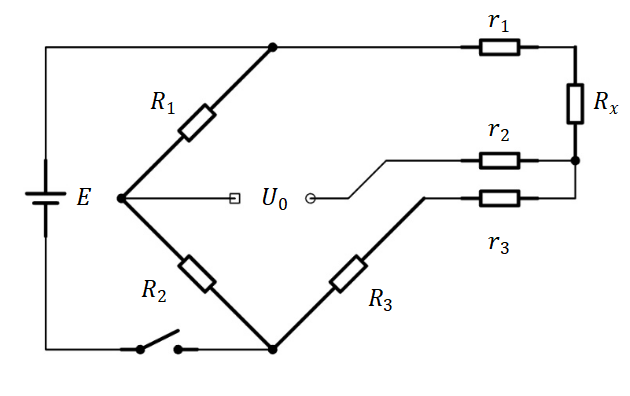
\includegraphics[width=0.6\textwidth]{image.png} 
    \caption{三线式非平衡电桥电路图}
    \label{fig:three_wire_unbalanced_bridge}
\end{figure}

在图\ref{fig:three_wire_unbalanced_bridge}所示电路中, 三根粗细, 长短均相同的导线电阻为$r_1$, $r_2$, $r_3$
与电阻$R_x$相连, 由于测量仪表电阻很大, 故$r_2$处电阻可以忽略, 而$r_1$与$r_3$与电桥的两臂相连, 
这样就消除了引线电阻对测量的影响. 

\subsection{心得体会}
这部分实验用到的热学实验仪的温度在达到设定温度之后不会立刻停下, 
而是会在温度超过几度后再回降到设定的温度
有时候会在设定温度附近反复振荡
这可能是由于虽然加热电流已经变成0,
但是加热装置上仍有一定的余热导致温度继续上升
实际实验的时候, 我们只需要在温度处在一个比较稳定的状态下就可以读取数值了, 
不必非要等到温度达到设定温度再读取数值, 由此可以提高实验效率. 

在实验中我发现在测量热电偶的温差电动势的时候, 由于热电偶的位置不够稳定,
电动势的读数会有较大的波动, 这可能会导致我测量结果的较大偏差. 因此我认为
如果能在实验中使用更加稳定的支架来固定热电偶, 同时增加冰水混合物中的冰块数量,
并尽快进行测量, 可能会减小误差.

在非平衡电桥温度计设计的实验中, 为了得到最后的实验参数需要进行大量计算,
为了减少误差, 我们尽量不要自行记录保留小数的中间结果, 最好使用Python
或者Matlab等科学计算工具将最精确的中间结果直接存储在变量中, 写好完整的代码
是得我们能直接输出结果, 这可以避免由于中间结果近似带来的误差, 从而提高实验的准确性.
\section{附录}

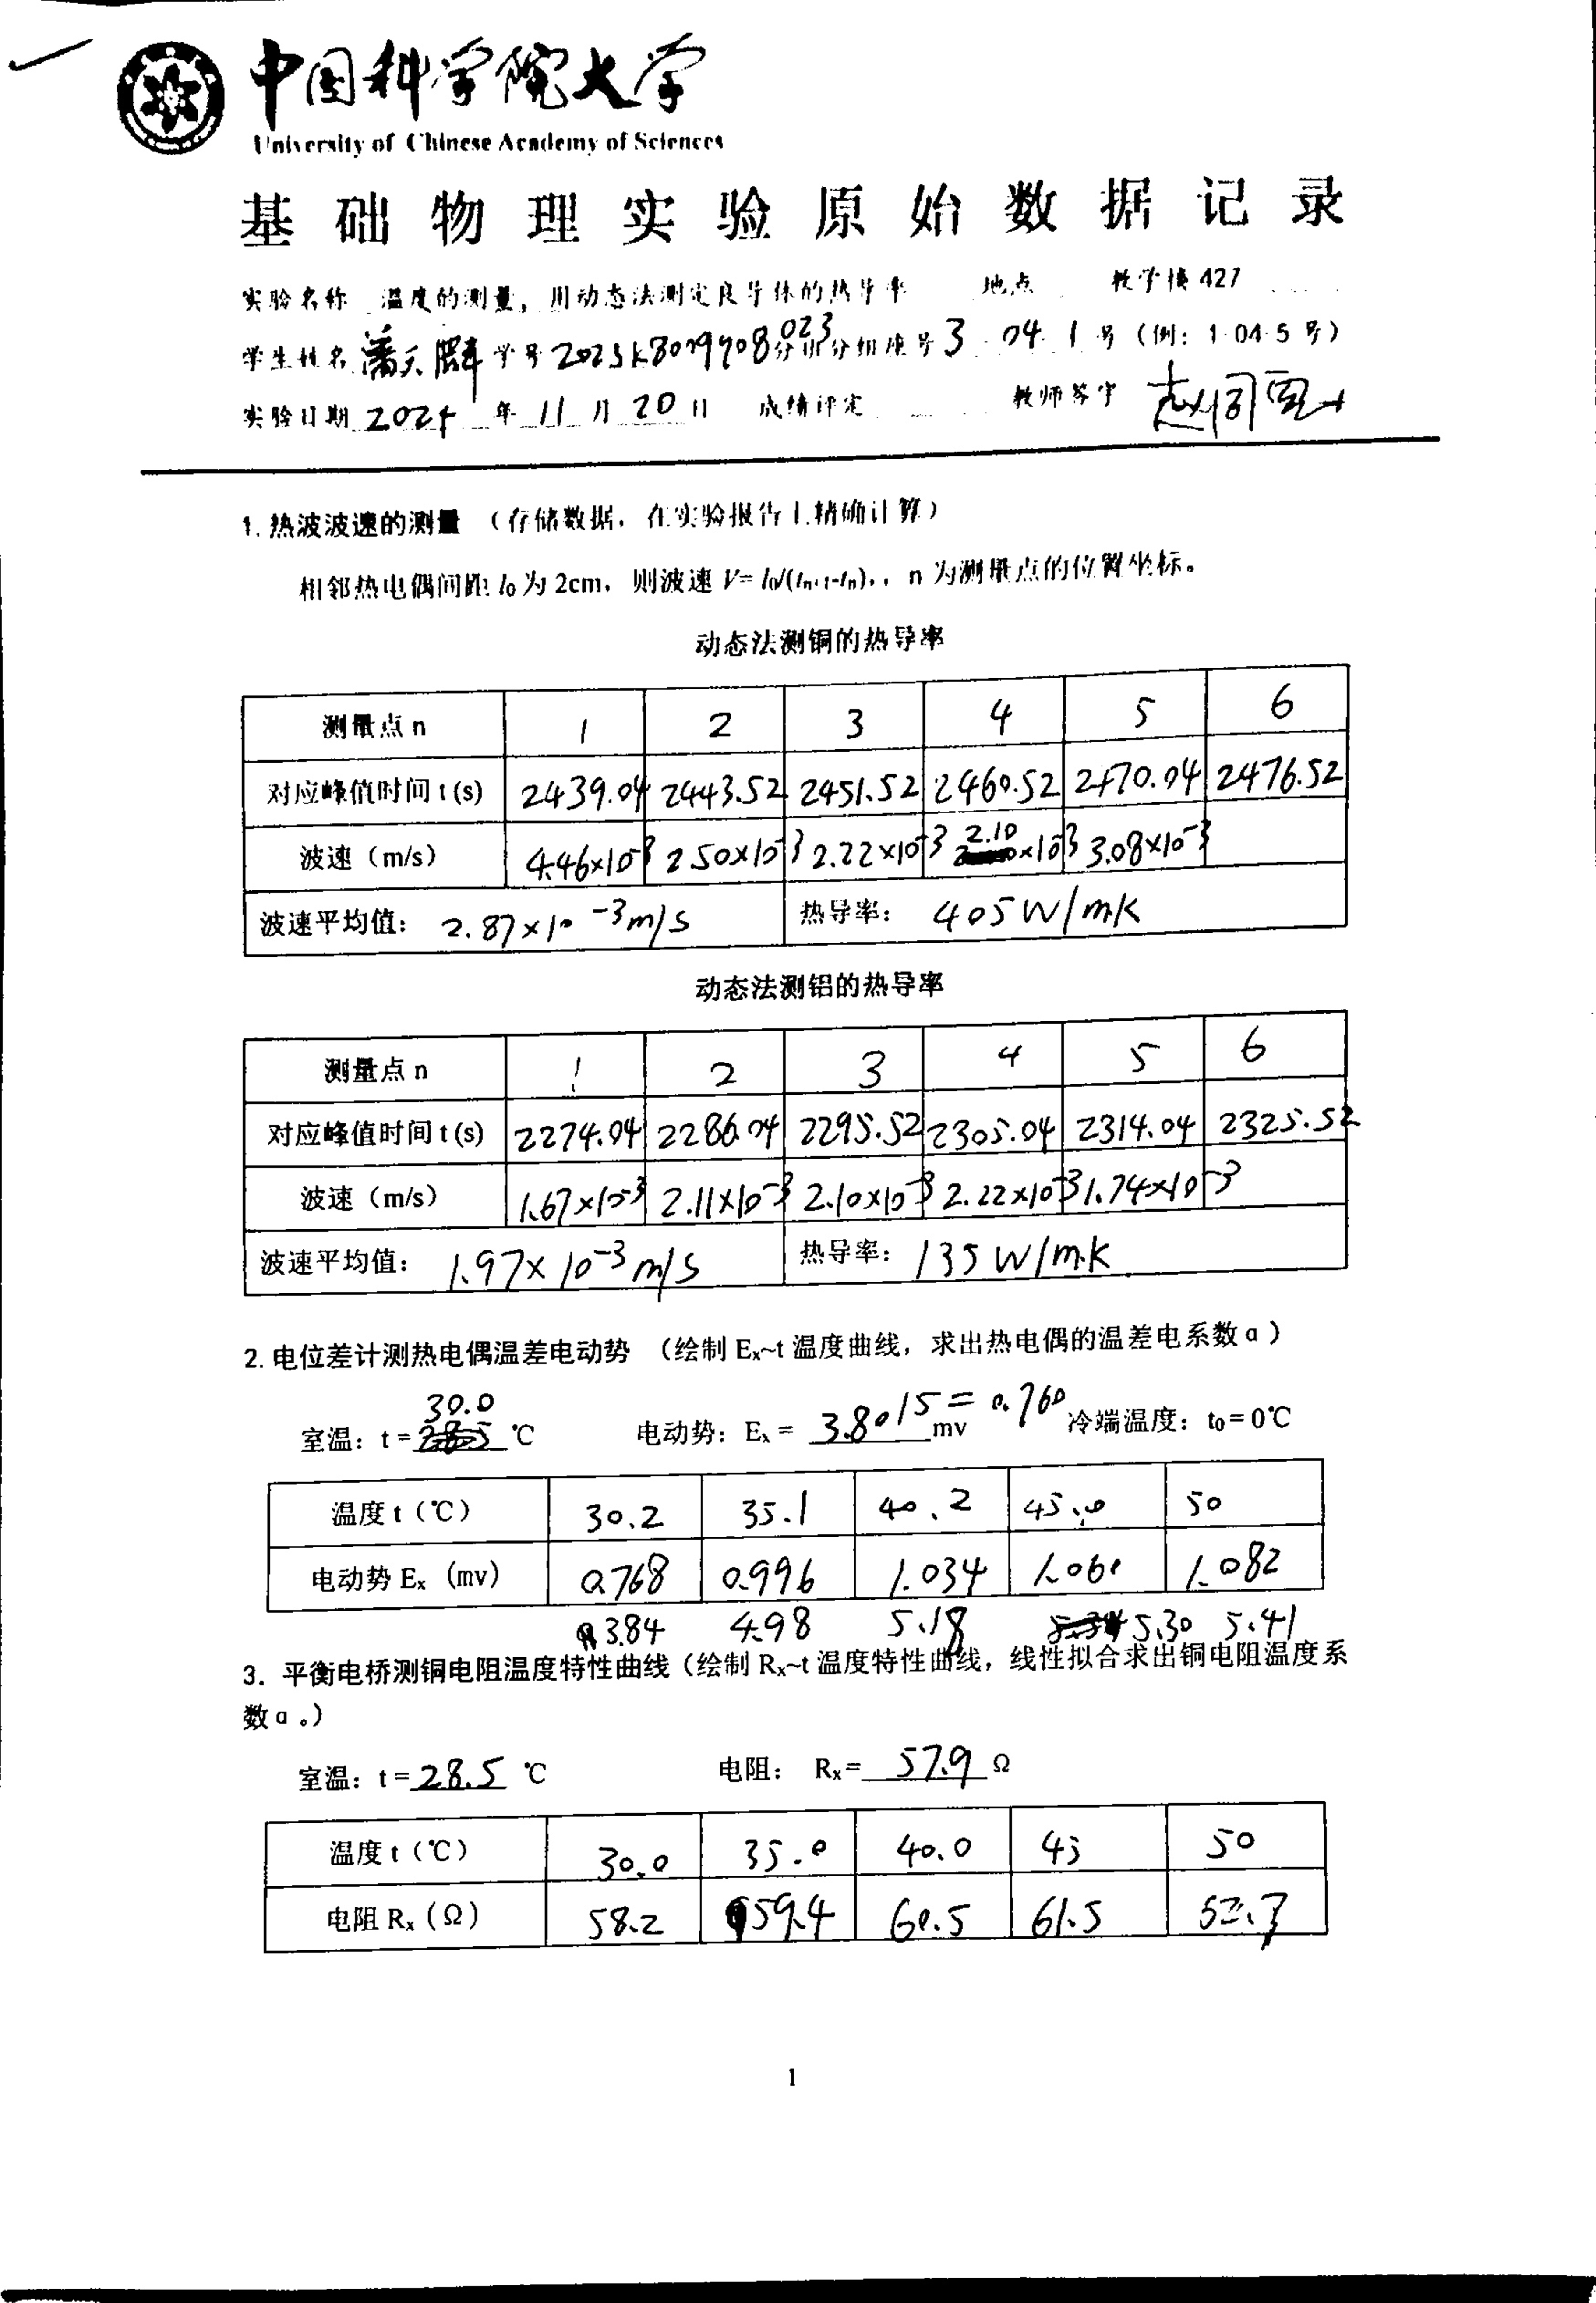
\includepdf[pages=-]{潘天麟-热导温度测量-数据.pdf}
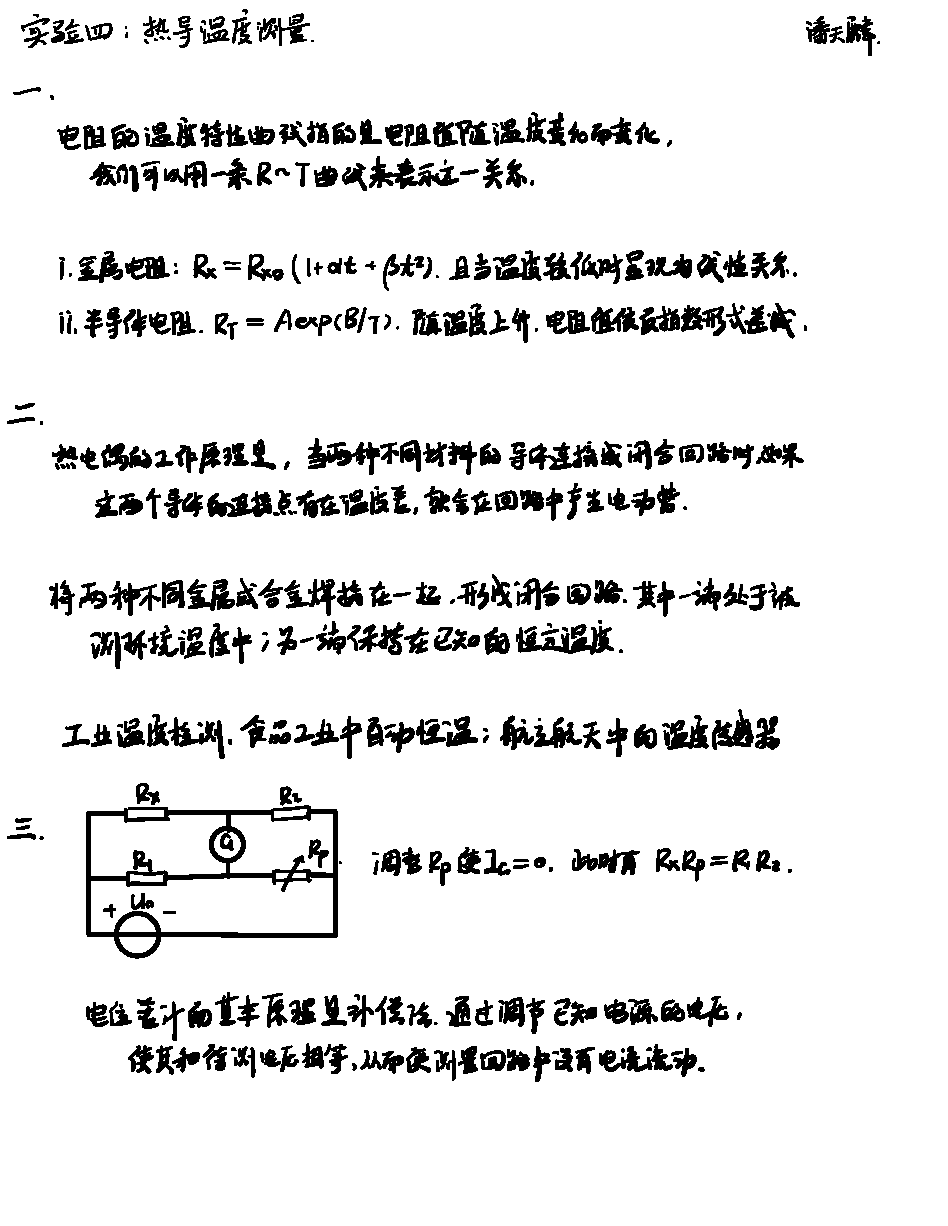
\includepdf[pages=-]{潘天麟-2024-11-20-热导温度测量-预习报告.pdf}
\end{document}
